\section{Compare economies and changes over time}
\subsection{Predict, plot, interpret}

\begin{frame}{The policy question contains two comparisons}
  \begin{enumerate}
    \item Do lower-income and higher-income economy--years occupy different
      parts of the mortality distribution?
    \item As the same economy changes over time, does its trajectory move in
      the same direction as the pooled association?
  \end{enumerate}

  \vspace{0.7em}
  The pooled scatterplot addresses the first comparison. Economy trajectories
  display the second.

  \vfill
  State the comparison before choosing the graph.
\end{frame}

\begin{frame}{Predict the pooled relationship}
  \begin{columns}[T,onlytextwidth]
    \column{0.76\textwidth}
      \textbf{Slido multiple choice}

      We will plot all 4,296 economy--years and use logarithmic scales on both
      axes. Which pattern do you expect?
      \begin{enumerate}
        \item A downward band with substantial dispersion.
        \item A downward band with nearly identical paths across economies.
        \item A flat cloud after the logarithmic transformations.
        \item Twenty-three separate bands, one for each year.
      \end{enumerate}

      \vspace{0.25em}
      Record your prediction. We will compare it with the plot.
    \column{0.20\textwidth}
      \onslide<1->{%
  \begin{center}
    \href{https://sli.do/2209653}{%
      
\includegraphics[width=2.45cm]{figures/slido-lesson-3-qr.png}%
    }

    \vspace{0.25em}
    {\scriptsize\href{https://sli.do/2209653}{\textbf{Join at sli.do}}\par}
    {\small\texttt{\#2209653}\par}
  \end{center}%
}

  \end{columns}
\end{frame}

\begin{frame}[fragile]{Build the pooled plot in RStudio}
\begin{lstlisting}[language=R]
ggplot(
  health_panel,
  aes(
    x = gdp_per_capita_ppp,
    y = under5_mortality
  )
) +
  geom_point(alpha = 0.34) +
  scale_x_log10() +
  scale_y_log10()
\end{lstlisting}

\end{frame}

\begin{frame}{Higher income is associated with lower under-five mortality}
  \centering
  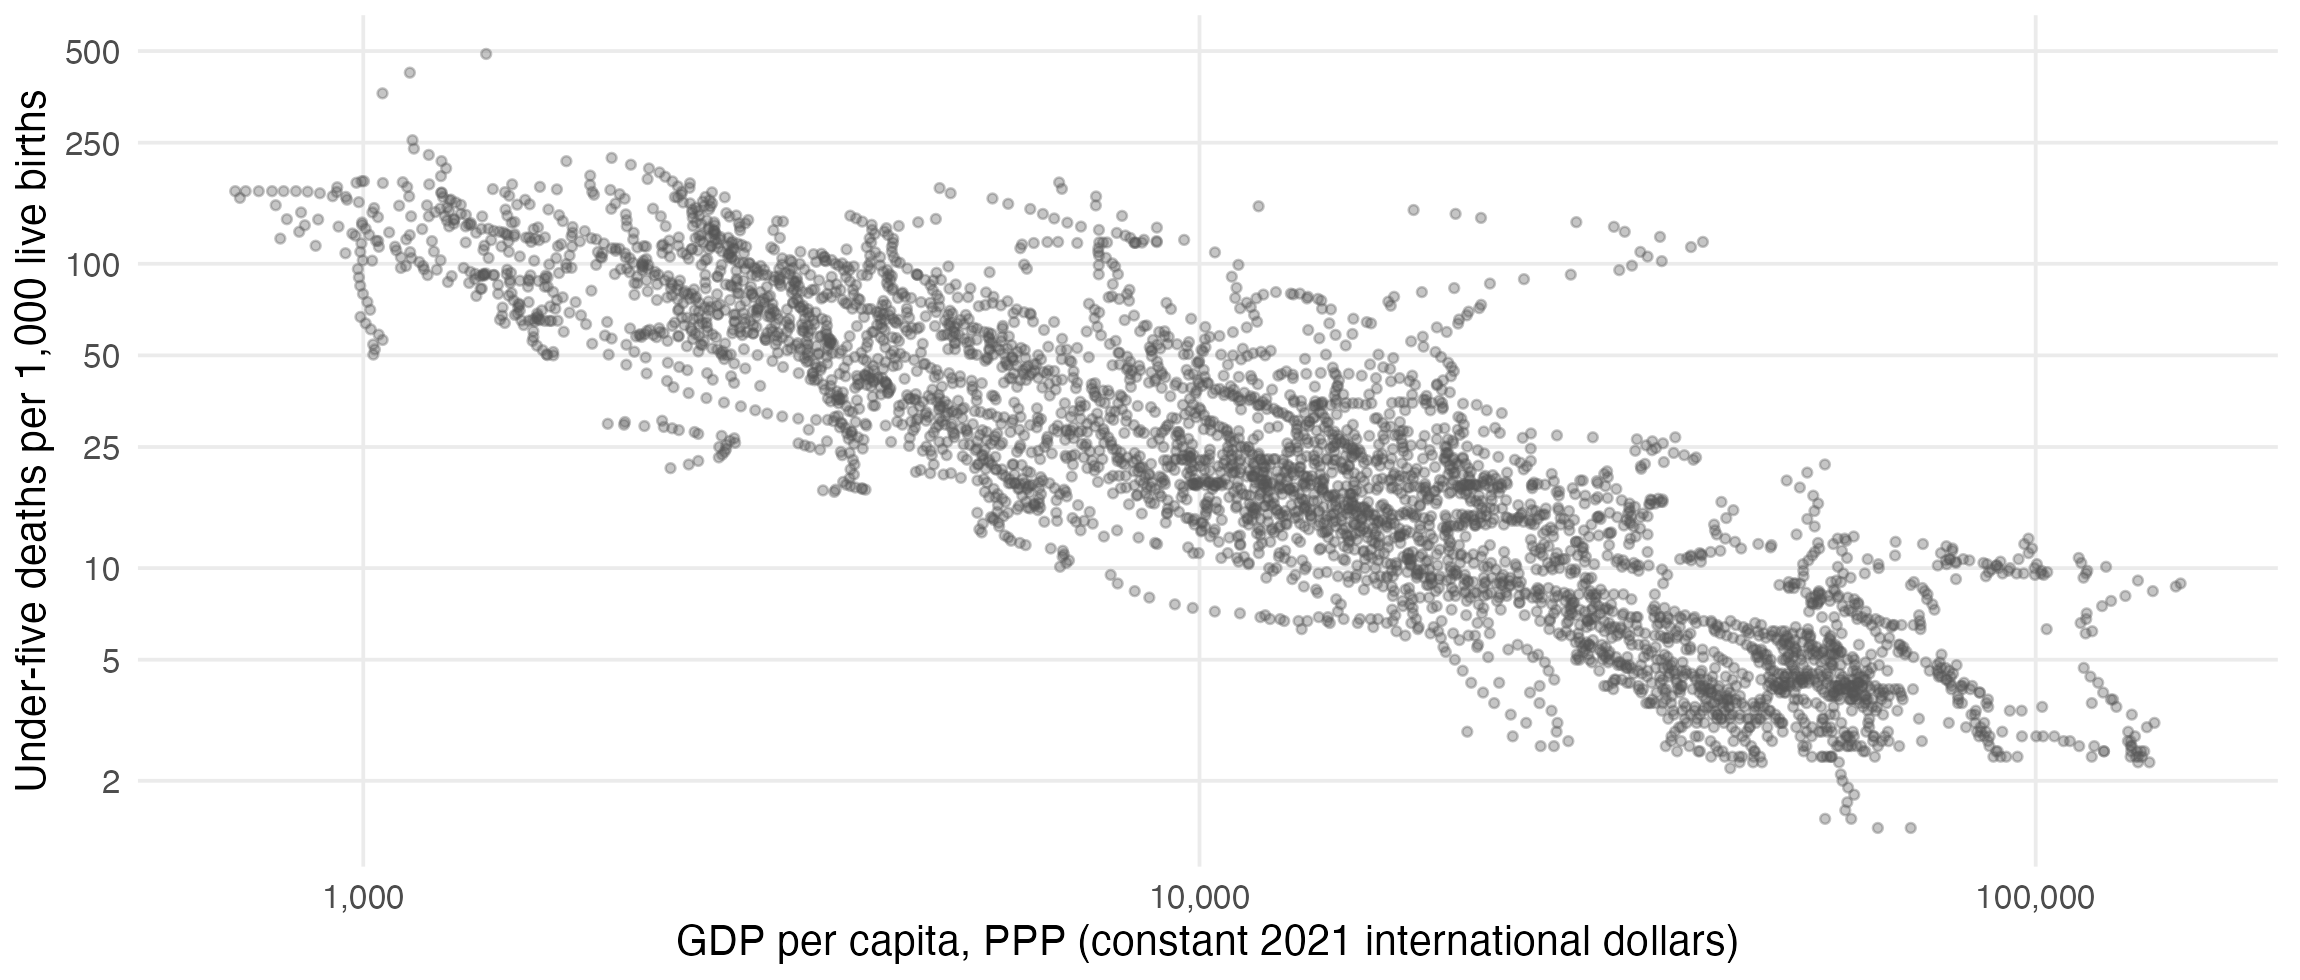
\includegraphics[width=0.92\textwidth,keepaspectratio]{figures/01-full-panel.png}
  \fnote{Source: World Bank, World Development Indicators. Each point is one
  observed economy--year from 2000--2022. Both axes use logarithmic scales.}
\end{frame}

\begin{frame}{Read the pooled plot}
  \begin{description}
    \item[Direction] Higher GDP per capita is associated with lower under-five mortality.
    \item[Dispersion] Economies at similar income levels can have substantially different mortality.
    \item[Departure] Some observations have much higher mortality than the pooled pattern predicts.
  \end{description}

  \vfill
  The plot establishes a descriptive association. Causal interpretation would
  require an identification strategy and evidence on competing explanations.
\end{frame}

\begin{frame}{Logarithmic axes represent proportional differences}
  Equal ratios receive equal visual distances:
  \[
    1{,}000 \rightarrow 2{,}000
    \qquad\text{and}\qquad
    50 \rightarrow 100.
  \]

  \begin{itemize}
    \item Income spans more than two orders of magnitude.
    \item Mortality ranges from roughly 1.4 to nearly 500 deaths per 1,000.
    \item The briefing concerns proportional differences in income and mortality.
  \end{itemize}

  \vfill
  Axis labels remain in the original units. The spacing is logarithmic.
\end{frame}

\begin{frame}{Each economy contributes repeated observations}
  In the pooled plot, an economy can appear up to 23 times. The point cloud
  combines:
  \begin{itemize}
    \item persistent differences across economies;
    \item changes within economies over time;
    \item common movements between 2000 and 2022;
    \item modest differences in annual coverage.
  \end{itemize}

  \vfill
  The pooled association draws on both cross-sectional and longitudinal
  variation.

  \vspace{0.35em}
  Before plotting the six trajectories, predict whether every selected economy
  will move along the pooled association.
\end{frame}

\begin{frame}{Six economy trajectories show the longitudinal variation}
  \vspace{0.35em}
  \centering
  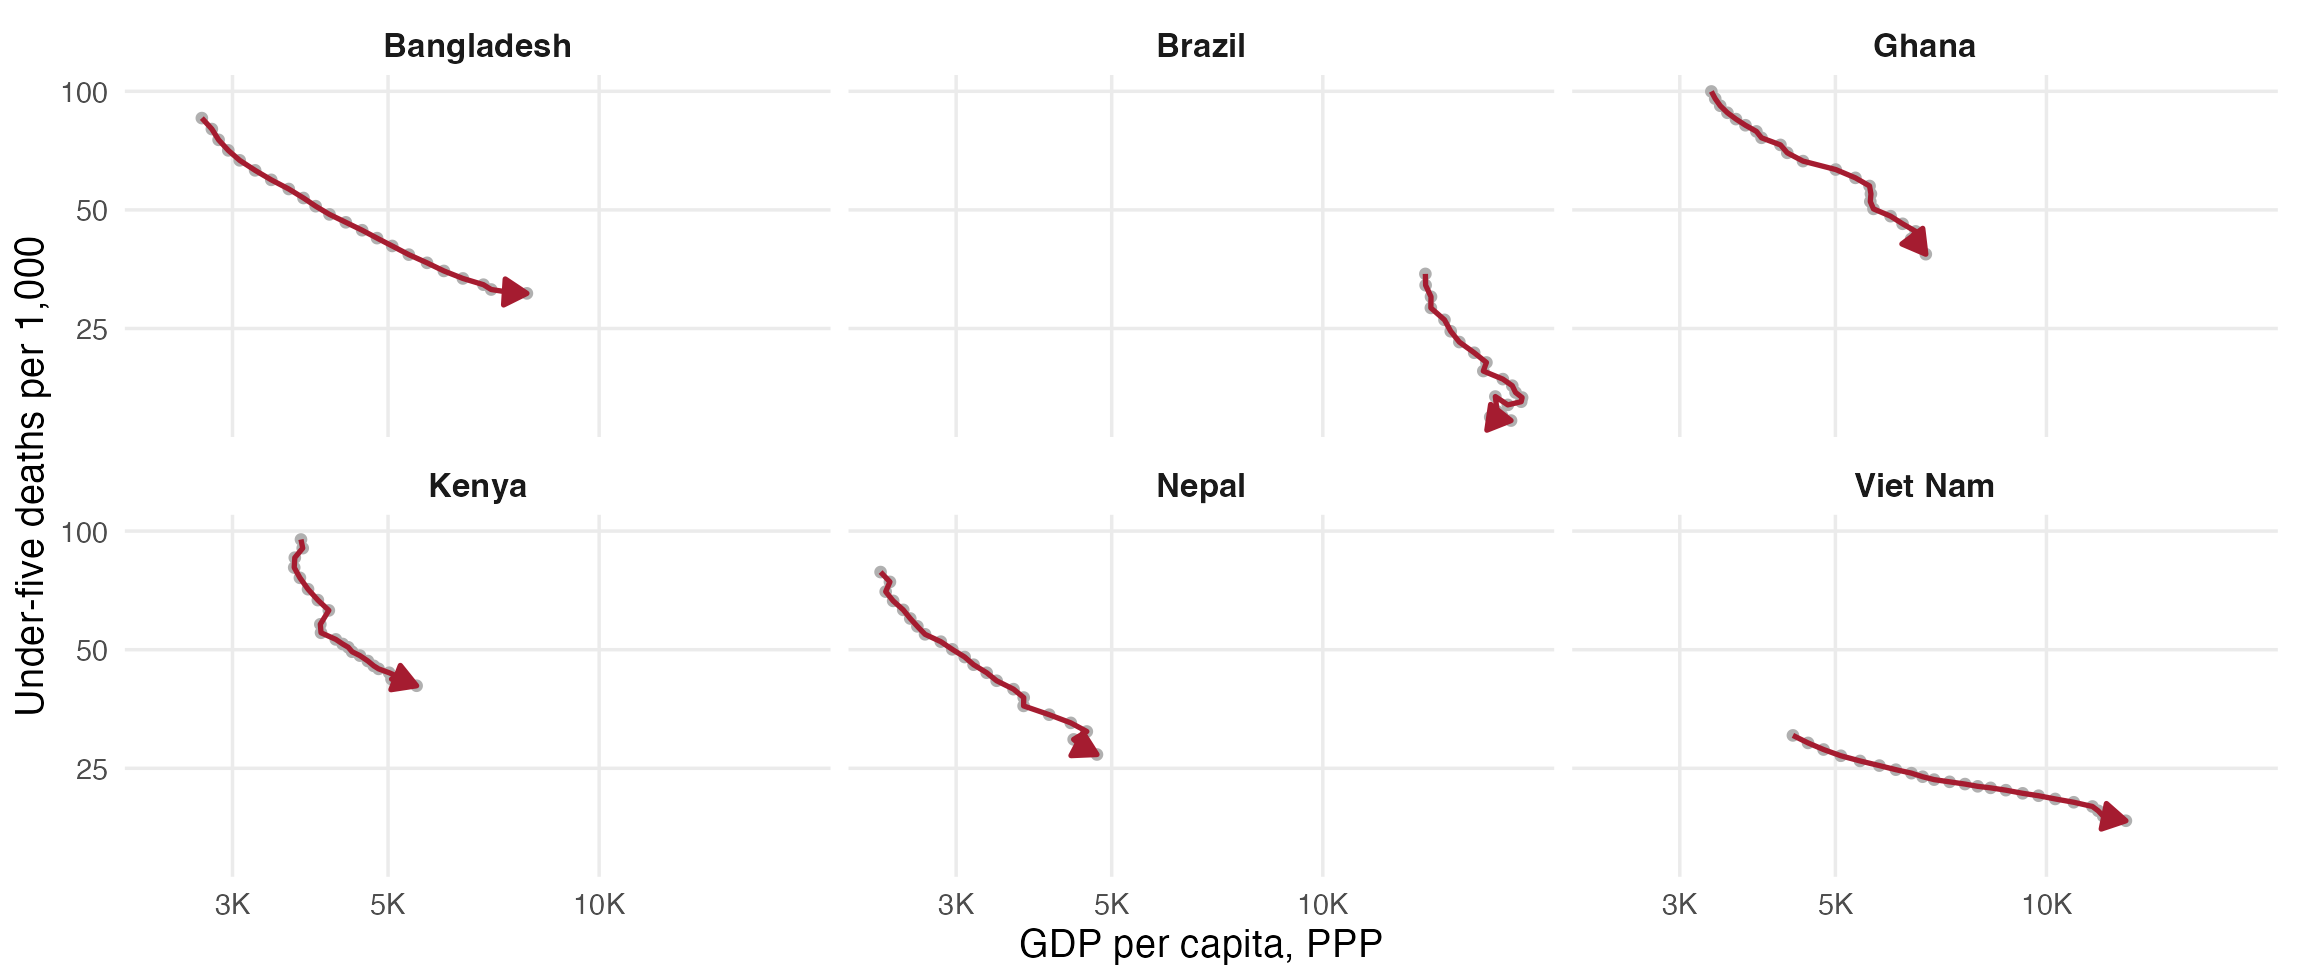
\includegraphics[width=0.91\textwidth,keepaspectratio]{figures/02-selected-trajectories.png}
  \fnote{Source: World Bank, World Development Indicators. Arrows follow each
  economy from earlier to later observed years.}
\end{frame}

\begin{frame}{The two figures use different comparisons}
  \small
  \begin{tabularx}{\textwidth}{@{}>{\bfseries\raggedright\arraybackslash}p{0.17\textwidth}>{\raggedright\arraybackslash}X>{\raggedright\arraybackslash}X@{}}
    \toprule
      & \textbf{Pooled plot} & \textbf{Economy trajectories} \\
    \midrule
    Unit shown & Economy--year & Repeated observations for one economy \\
    \addlinespace[0.35em]
    Comparison & Higher-income and lower-income observations & Earlier and later observations within an economy \\
    \addlinespace[0.35em]
    Use & Describe the overall association and dispersion & Document heterogeneity in changes over time \\
    \addlinespace[0.35em]
    Limitation & Combines between- and within-economy variation & Selected economies do not summarize the full sample \\
    \bottomrule
  \end{tabularx}

  \vfill
  The models will state which comparisons contribute to each coefficient.
\end{frame}

\begin{frame}{Checkpoint 1: answer the director}
  A director sees the pooled plot and says: ``Economic growth reduces child
  mortality. We should put that in the briefing.''

  \vspace{0.5em}
  \begin{enumerate}
    \item one claim the plot supports;
    \item one reason the causal sentence exceeds the evidence;
    \item one potential analysis we would like to implement.
  \end{enumerate}

  \vfill
  \centering
  \textbf{2 minutes discuss}\qquad$\longrightarrow$\qquad
  \textbf{2 minutes share}
\end{frame}

\begin{frame}{Checkpoint 1: model response}
  \begin{enumerate}
    \item \textbf{Supported claim:} Across observed economy--years during
      2000--2022, higher GDP per capita is associated with lower under-five
      mortality.
    \item \textbf{Causal gap:} The specification does not isolate exogenous
      variation in income. Health systems, institutions, conflict, inequality,
      and other determinants can change with income.
    \item \textbf{Next comparison (potential analysis):} Changes within the same economy after
      accounting for common year movements.
  \end{enumerate}

\end{frame}

\begin{frame}[plain]{Ten-minute break}
  \vfill
  \begin{center}
    {\LARGE\color{crimson}Return in ten minutes.}\par
    \vspace{0.5em}
    Leave the Lesson 3 walkthrough open at Section 4 in RStudio.
  \end{center}
  \vfill
\end{frame}
